\documentclass[11pt]{article}

\usepackage[a4paper,margin=2.4cm]{geometry}
\usepackage{amsmath,amssymb,amsthm}
\usepackage{graphicx}
\usepackage{booktabs}
\usepackage{xcolor}
\usepackage[hidelinks]{hyperref}

\graphicspath{{data/output/}{../data/output/}}

\DeclareMathOperator{\tr}{tr}
\DeclareMathOperator{\Var}{Var}
\DeclareMathOperator{\Cov}{Cov}
\newcommand{\R}{\mathbb{R}}
\newcommand{\Xt}{\widetilde{X}}
\newcommand{\xt}{\widetilde{x}}
\newcommand{\Nt}{\widetilde{N}}
\newcommand{\norm}[1]{\lVert #1 \rVert}
\newcommand{\T}{^{\mathsf{T}}}

\theoremstyle{definition}
\newtheorem{definition}{Definition}[section]
\theoremstyle{plain}
\newtheorem{proposition}{Proposition}[section]
\theoremstyle{remark}
\newtheorem{remark}{Remark}[section]

\title{\bfseries Linear-Algebraic Analysis of a High-Dimensional\\ Spectroscopic Dataset:\\ Cleaning, Principal Component Analysis, and Clustering}
\author{SIMC 2026 Endeavour Challenge --- Question 3, Parts (a)--(e)}
\date{May 2026}

\begin{document}
\maketitle

\begin{abstract}
\noindent
We analyse a design matrix of $N=1000$ infrared spectra, each recorded at $M=3401$
frequencies. We first remove two classes of corrupted measurements by thresholding the
distribution of row norms at its spectral gaps, retaining $\Nt=924$ clean spectra. After
mean-centering we form the covariance matrix $C=\tfrac1{\Nt}\Xt\T\Xt$ and prove that its
diagonal records the per-feature variances and that its trace, the total variance, is
conserved under orthogonal change of basis. Diagonalising $C$ (principal component
analysis) yields a spectrum with a sharp elbow at $k^\star=8$ signal eigenvalues and a
dominance ratio $\lambda_1/\lambda_2\approx3.53$; we show that the conventional
``$95\%$ of variance'' rule is misleading here, requiring $667$ mostly-noise components.
The leading eigenvector is a contrast direction supported on two narrow molecular bands and
is shown to be a difference-spectrum, essentially orthogonal to the mean spectrum.
Projecting the data onto the four leading eigenvectors resolves the samples into
approximately $25$ well-separated clusters, each a distinct chemical concoction.
\end{abstract}

\section{Setup and notation}\label{sec:setup}

The data form a \emph{design matrix} $X\in\R^{N\times M}$ whose rows are \emph{samples}
(one vial of a liquid sample) and whose columns are \emph{features} (one infrared
frequency). The entry $X_{ij}$ is the absorbance of sample $i$ at frequency $j$. We take
$N=1000$ and $M=3401$.

\begin{remark}
The problem statement quotes $M=3041$, whereas the supplied array
\texttt{mystery\_matrix1.npy} has a $3401$-long feature axis; the two figures are a digit
transposition. We trust the data and use $M=3401$ throughout, identifying the sample axis
as the one of length $1000$. The file is stored transposed (shape $3401\times1000$), so we
work with its transpose so that rows index samples.
\end{remark}

\begin{definition}[Euclidean norm]
For $x=(x_1,\dots,x_M)\in\R^M$, the Euclidean norm is
$\norm{x}=\bigl(\sum_{j=1}^M x_j^2\bigr)^{1/2}$, the length of $x$. It is a single scalar
summarising the overall magnitude of a spectrum.
\end{definition}

\section{Part (a): cleaning the data}\label{sec:clean}

\subsection*{Empty vials}
A vial containing no sample yields only low-amplitude background noise: a nearly flat
spectrum of small values and hence a small norm. A genuine spectrum has sharp absorption
peaks and a large norm. Sorting the $1000$ row norms exposes a clean gap: $40$ measurements
lie at $\norm{x}\approx1.6$, after which there is a void until the bulk begins at
$\norm{x}\approx4.3$ (Figure~\ref{fig:clean}, left). We set the threshold at the midpoint of
this largest sub-median gap, a choice that requires no hand-tuned constant and is stable
under perturbation. This isolates exactly $T=40$ empty vials, which are precisely rows
$960$--$999$.

\subsection*{A second error: high-norm outliers}
The upper tail of the norm distribution contains a second, clearly detached group of $36$
measurements at $\norm{x}\approx8.9$, separated from the bulk by a gap roughly five times
wider than any internal gap and occupying the contiguous block of rows $924$--$959$. We flag
these as a second error. We note that a coherent high-magnitude group could also be a
genuinely strong concoction; we therefore (i) provide the independent evidence of
Section~\ref{sec:clusters} that they form a single isolated cluster whose removal lowers the
cluster count by exactly one, and (ii) keep the removal reversible.

\subsection*{Selection by Boolean mask}
Writing $\mathbf{1}[\cdot]$ for the indicator, we retain sample $i$ iff
$\tau_{\mathrm{lo}}\le\norm{x_i}\le\tau_{\mathrm{hi}}$ with
$\tau_{\mathrm{lo}}\approx2.98$, $\tau_{\mathrm{hi}}\approx8.15$. Indexing by this Boolean
mask (rather than deleting rows) is non-destructive, composes the two criteria in one
operation, and preserves original sample indices. The cleaned matrix has $\Nt=924$ rows.

\subsection*{Validation}
The removed spectra are flat noise, the retained ones peaked. Quantitatively, the empty
vials are $50.2\%$ exact zeros against $24.5\%$ for genuine spectra: background noise is
symmetric about zero and the instrument clips negative absorbance to zero, so a zero-mean
noise channel is exactly $0$ with probability $\approx\tfrac12$, a signature absent from
peak-bearing data.

\begin{figure}[h]
\centering

\includegraphics[width=0.92\linewidth]{q3a_part_i.png}\\[2pt]

\includegraphics[width=0.62\linewidth]{q3a_part_ii_clusters.png}
\caption{\emph{Top:} row-norm distribution; $40$ empty vials sit below the gap, with example
empty (flat) and genuine (peaked) spectra. \emph{Bottom:} the $36$ high-norm vials form one
tight, isolated cluster in the leading principal-component plane.}
\label{fig:clean}
\end{figure}

\section{Part (b): variance, mean-centering, and the covariance matrix}\label{sec:cov}

\begin{definition}[Mean-centering]
With column means $\bar X_j=\tfrac1{\Nt}\sum_{i=1}^{\Nt}X_{ij}$, the centered matrix is
$\Xt_{ij}=X_{ij}-\bar X_j$, so every feature has zero mean.
\end{definition}

Mean-centering is essential: without it the dominant direction of variation would be the
mean spectrum shared by all samples, which carries no discriminative information. We study
deviations from the mean, where the discriminating structure lives.

\begin{definition}[Covariance matrix]
$\displaystyle C=\tfrac1{\Nt}\,\Xt\T\Xt\in\R^{M\times M}$, with
$C_{ij}=\tfrac1{\Nt}\sum_{k=1}^{\Nt}\Xt_{ki}\Xt_{kj}$.
\end{definition}

\begin{proposition}\label{prop:diag}
$C$ is symmetric, and its diagonal entries are the per-feature variances:
$C_{jj}=\Var_j:=\tfrac1{\Nt}\sum_{k}\Xt_{kj}^2$.
\end{proposition}
\begin{proof}
Symmetry: $C\T=\tfrac1{\Nt}(\Xt\T\Xt)\T=\tfrac1{\Nt}\Xt\T\Xt=C$. Setting $i=j$ in the
definition gives $C_{jj}=\tfrac1{\Nt}\sum_k\Xt_{kj}^2$, which, as the data are centered, is
exactly the variance of feature $j$.
\end{proof}

\begin{proposition}[Conservation of total variance]\label{prop:trace}
The total variance $\tr(C)=\sum_j C_{jj}$ is invariant under any orthogonal change of basis
$C\mapsto Q\T C Q$ ($Q\T Q=I$); in particular it equals the sum of the eigenvalues of $C$.
\end{proposition}
\begin{proof}
$\tr(Q\T C Q)=\tr(C QQ\T)=\tr(C)$ by cyclicity of the trace and $QQ\T=I$. Diagonalising
$C=Q\Lambda Q\T$ gives $\tr(C)=\tr(\Lambda)=\sum_i\lambda_i$.
\end{proof}

Empirically $\tr(C)\approx7.90$. The variance profile (Figure~\ref{fig:var}) is concentrated
in a few narrow bands --- the molecular absorption regions --- with the global maximum at
feature $j^\star=910$, where $C_{j^\star j^\star}\approx0.0199$. Most features are nearly
flat, so the data is effectively low-dimensional.

\begin{figure}[h]
\centering

\includegraphics[width=\linewidth]{q3b_variance.png}
\caption{Per-feature variance $C_{jj}$. Variance concentrates in narrow molecular bands; the
red line marks the maximal-variance feature $j^\star=910$.}
\label{fig:var}
\end{figure}

\section{Part (c): the eigenspectrum (PCA)}\label{sec:pca}

\begin{definition}[Eigenpair]
$(\lambda,\nu)$ with $\nu\neq0$ is an eigenpair of $C$ if $C\nu=\lambda\nu$.
\end{definition}

\begin{proposition}[Eigenvalues are variances]\label{prop:rayleigh}
For a unit vector $w$, the variance of the data projected onto $w$ is $w\T C w$. If
$C\nu=\lambda\nu$ with $\norm{\nu}=1$ then $\nu\T C\nu=\lambda$.
\end{proposition}
\begin{proof}
The projection of sample $\xt_i$ onto $w$ is $z_i=\xt_i\!\cdot w$, with mean zero; its
variance is $\tfrac1{\Nt}\sum_i z_i^2=\tfrac1{\Nt}w\T\Xt\T\Xt w=w\T C w$. Substituting
$C\nu=\lambda\nu$ and $\norm{\nu}=1$ gives $\nu\T C\nu=\lambda\norm{\nu}^2=\lambda$.
\end{proof}

\begin{proposition}\label{prop:psd}
$C$ is positive semi-definite; hence all $\lambda_i\ge0$.
\end{proposition}
\begin{proof}
For any $w$, $w\T C w=\tfrac1{\Nt}\norm{\Xt w}^2\ge0$. Applying this to a unit eigenvector
and using Proposition~\ref{prop:rayleigh} gives $\lambda=\nu\T C\nu\ge0$.
\end{proof}

By the spectral theorem $C$ (real symmetric) has real eigenvalues and an orthonormal
eigenbasis. We compute the decomposition with \texttt{numpy.linalg.eigh}, which is
specialised for symmetric matrices --- guaranteeing real eigenvalues and orthonormal
eigenvectors, and faster and more stable than \texttt{eig} --- then sort the eigenvalues in
decreasing order and clip rounding-level negatives to zero (justified by
Proposition~\ref{prop:psd}).

\begin{table}[h]
\centering
\begin{tabular}{lrrrrrrrrr}
\toprule
$k$ & 1 & 2 & 3 & 4 & 5 & 6 & 7 & 8 & 9\\
\midrule
$\lambda_k$ & 2.492 & 0.705 & 0.590 & 0.254 & 0.123 & 0.105 & 0.078 & 0.039 & 0.0093\\
\bottomrule
\end{tabular}
\caption{Leading eigenvalues. The drop $\lambda_8/\lambda_9\approx4.1$ is the largest in the
spectrum and marks the signal/noise boundary.}
\label{tab:eig}
\end{table}

\subsection*{Dominance ratio and the elbow}
The dominance ratio is $\lambda_1/\lambda_2\approx3.53$: one direction captures far more
variance than any other, indicating strong low-dimensional structure (and a wide spectral
gap, the condition for rapid convergence of the Power Method of Question 2). We locate the
\emph{elbow} as the largest multiplicative drop between consecutive eigenvalues --- a ratio,
since the signal/noise transition is multiplicative on the logarithmic scale of
Figure~\ref{fig:scree}. The maximal drop is $\lambda_8/\lambda_9\approx4.1$
(Table~\ref{tab:eig}), giving $k^\star=8$: $\lambda_8$ remains $\approx4\times$ above the
noise floor (signal), while $\lambda_9$ already lies on the floor (noise). This agrees with
the $\sim10$ dominant molecules: a few chemical components span only a few independent
directions.

\begin{figure}[h]
\centering

\includegraphics[width=\linewidth]{q3c_spectrum.png}
\caption{Eigenvalue spectrum on linear (left) and logarithmic (right) scales. The logarithmic
plot exhibits a sharp elbow at $k^\star=8$, followed by a flat noise floor.}
\label{fig:scree}
\end{figure}

\subsection*{Cumulative variance: a caution}
Let the explained-variance ratio be $\lambda_k/\sum_i\lambda_i$. The eight signal components
account for only $\approx55.5\%$ of the total variance; reaching $95\%$ requires $k=667$
components (Table~\ref{tab:cum}, Figure~\ref{fig:cum}). The reason is that the small noise
floor is spread over $\approx900$ dimensions (the rank is at most $\Nt-1$), so its tiny
per-component contributions accumulate. The naive ``retain $95\%$ of variance'' heuristic
therefore grossly overestimates the dimensionality; the elbow $k^\star=8$ is the honest
measure. As a check, $\sum_i\lambda_i\approx\tr(C)\approx7.90$
(Proposition~\ref{prop:trace}).

\begin{table}[h]
\centering
\begin{tabular}{lrrrrr}
\toprule
cumulative variance & $50\%$ & $80\%$ & $90\%$ & $95\%$ & $99\%$\\
\midrule
components $k$ & 4 & 309 & 516 & 667 & 850\\
\bottomrule
\end{tabular}
\caption{Components required to reach each variance threshold; contrast the $8$ signal
components ($55.5\%$) with the $667$ needed for $95\%$.}
\label{tab:cum}
\end{table}

\begin{figure}[h]
\centering

\includegraphics[width=0.95\linewidth]{q3c_cvarr.png}
\caption{Cumulative variance versus $k$. The elbow (red) reaches only $\approx55\%$;
$95\%$ (green) is not attained until $k=667$.}
\label{fig:cum}
\end{figure}

\section{Part (d): the leading eigenvector}\label{sec:lead}

The leading eigenvector $\nu_1\in\R^M$ lies in feature space and assigns a \emph{loading} to
each frequency; equivalently it is the direction of greatest variance. The associated
\emph{scores} $z_i=\xt_i\!\cdot\nu_1$ are, by Proposition~\ref{prop:rayleigh}, the
maximally-spread one-dimensional summaries of the samples. Eigenvectors are defined only up
to sign ($C(-\nu)=\lambda(-\nu)$); we fix the sign so the largest-magnitude loading is
positive.

Figure~\ref{fig:lead} (left) shows that $\nu_1$ is supported on two narrow bands
($j\approx900$--$960$ and $j\approx3150$--$3260$) and takes both signs ($\approx27\%$ of
loadings negative). Mixed signs make $\nu_1$ a \emph{contrast}: it measures the balance of
absorption between two groups of frequencies rather than overall intensity.

\begin{definition}[Cosine similarity]
$\cos(a,b)=\dfrac{a\!\cdot b}{\norm{a}\,\norm{b}}\in[-1,1]$, the cosine of the angle between
$a$ and $b$; it is scale-invariant and compares direction, not magnitude.
\end{definition}

We find $\cos(\nu_1,\xt_{193})\approx0.92$ for the best-matching \emph{centered} spectrum,
but only $\approx0.67$ against the corresponding \emph{raw} spectrum and $\approx0.03$
against the mean spectrum. Because $\nu_1$ lives in the centered space it is essentially
orthogonal to the (uncentered) mean, which dominates raw spectra; hence $\nu_1$ resembles a
\emph{difference-spectrum} --- the way the most-deviated concoction departs from the mean
(Figure~\ref{fig:lead}, right). This mirrors Question 1, where the dominant eigenvector was
the long-time steady state of the dynamics.

\begin{figure}[h]
\centering
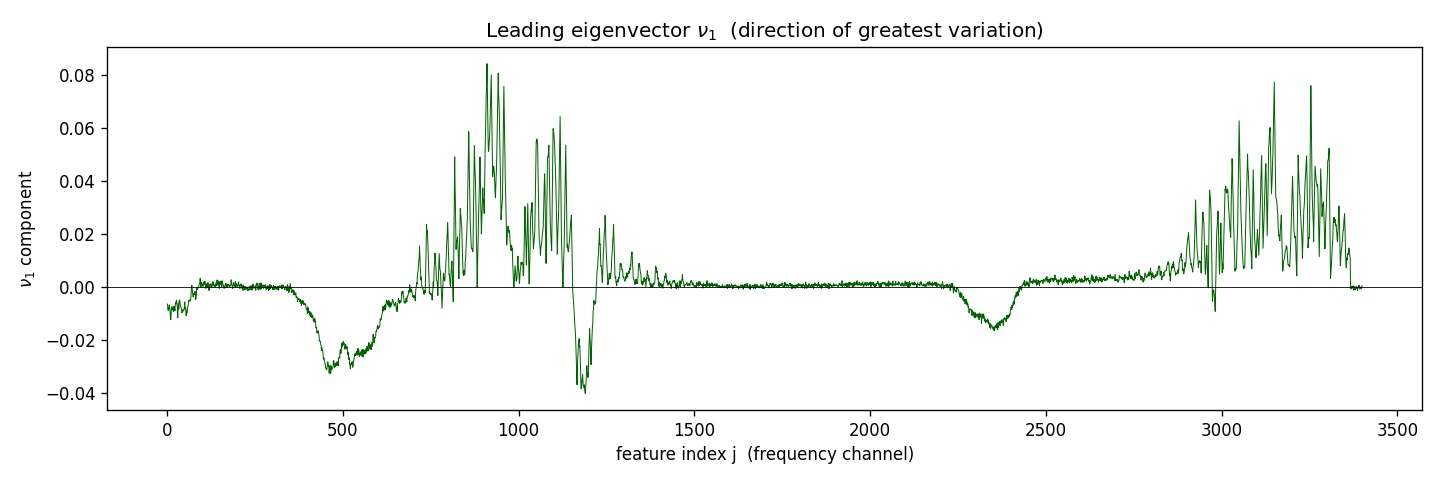
\includegraphics[width=0.85\linewidth]{q3d_v1.png}\\[2pt]

\includegraphics[width=0.85\linewidth]{q3d_v1_vs_row.png}
\caption{\emph{Top:} loadings of $\nu_1$, concentrated in two molecular bands with mixed
signs (a contrast direction). \emph{Bottom:} $\nu_1$ overlaid with the best-matching centered
spectrum ($\cos\approx0.92$).}
\label{fig:lead}
\end{figure}

\section{Part (e): clustering in covariance space}\label{sec:clusters}

We project onto the four leading eigenvectors. With $V_4=[\nu_1\,\nu_2\,\nu_3\,\nu_4]\in
\R^{M\times4}$, the compressed coordinates are $Z=\Xt V_4\in\R^{\Nt\times4}$; row $z_i$ holds
sample $i$'s four scores. This is dimensionality reduction from $3401$ to $4$ retaining the
dominant variation. The $\binom{4}{2}=6$ pairwise scatter plots (Figure~\ref{fig:scatter})
reveal many tight, well-separated groups.

To count them without external libraries we use leader clustering: traversing the points,
a new cluster centre is opened whenever a point lies farther than a radius $r$ from all
existing centres. With $r$ set to a few multiples of the median nearest-neighbour spacing the
count is stable at $25$ for all $r\in[6,12]\times$, so it reflects the data rather than the
threshold. Hence the $924$ cleaned vials comprise $\approx25$ distinct concoctions ---
comfortably below the ``fewer than $100$ unique samples'' of Part (h). Although $\nu_1,\dots,
\nu_4$ live in feature space, projecting samples onto them exposes structure in sample space,
because chemically similar spectra receive similar scores. Part (f) repeats the construction
with the Gram matrix $G=\tfrac1{\Nt}\Xt\Xt\T$, which shares the nonzero eigenvalues of $C$
(Question 2d) and should recover the same groups.

\begin{figure}[h]
\centering

\includegraphics[width=\linewidth]{q3e_covariance_scatter.png}
\caption{The six pairwise scatter plots of the top-4 principal-component scores. Each point
is one vial; the data resolves into $\approx25$ well-separated clusters.}
\label{fig:scatter}
\end{figure}

\section{Summary}\label{sec:summary}

Cleaning by norm-gap thresholding removed $40$ empty vials and $36$ high-norm outliers,
leaving $\Nt=924$ spectra. The covariance matrix has total variance $\tr(C)\approx7.90$, a
dominance ratio $\lambda_1/\lambda_2\approx3.53$, and a signal subspace of dimension
$k^\star=8$; the $95\%$-variance heuristic is shown to be inappropriate. The leading
eigenvector is an interpretable difference-spectrum, and projection onto the top four
eigenvectors resolves the data into $\approx25$ chemical concoctions. All computations are
reproduced in the accompanying notebook \texttt{SIMC\_2026.ipynb}.

\end{document}
